% =====================================================================
%  EvoApplications 2027 submission (double-blind)
%  Springer LNCS: put llncs.cls and splncs04.bst next to this file
%  (Overleaf's "Springer LNCS" template already has both).
% =====================================================================
\documentclass[runningheads]{llncs}

\usepackage[T1]{fontenc}
\usepackage{amsmath,amssymb}
\usepackage{booktabs}
\usepackage{graphicx}
\usepackage{tikz}
\usetikzlibrary{arrows.meta}
\usepackage{xcolor}
\usepackage{url}
\usepackage{hyperref}
\hypersetup{hidelinks}

% Red reminder for anything that must be checked before submission.
% Make it empty (\renewcommand{\chk}[1]{}) for the final PDF, then search for \chk.
\newcommand{\chk}[1]{\textcolor{red}{[#1]}}

\begin{document}

\title{Evolving Slot Machine Reel Strips Under Noisy Simulation:\\
When Does a Genetic Algorithm Beat Local Search?}
\titlerunning{Evolving Slot Machine Reel Strips Under Noisy Simulation}

% Double-blind: no names, affiliations or e-mail addresses.
\author{Anonymous Author(s)}
\authorrunning{Anonymous}
\institute{Anonymous Institution}

\maketitle

\begin{abstract}
\chk{Abstract, about 150 words, written last.}
\keywords{genetic algorithms \and noisy optimisation \and simulation-based optimisation \and game design \and slot machines}
\end{abstract}

% ---------------------------------------------------------------------
\section{Introduction}
\label{sec:intro}
\chk{Section 1: problem, why tuning is hard (cost per evaluation, noise), three contributions.}

% =====================================================================
%  Section 2 - Background: slot mathematics (author's draft, edited;
%  shortened 8 Nov for the page limit)
% =====================================================================
\section{Background: How a Video Slot Pays}
\label{sec:background}

The main backbone of a video slot is its reel set. A reel set has several reels, and each reel has a cyclic strip of $L$ symbols. The frequency and position of symbols on the strips decide how big and how frequent the wins can be. During a spin, the game stops each reel at a random position, independently and uniformly, and shows the symbol at the stop and the $N$ symbols below it (Fig.~\ref{fig:reels}).

In our case the reel set has 5 reels, each with a strip of length $L = 50$, i.e.\ $50^5 \approx 3.1 \times 10^8$ equally likely stop combinations, and we show $N = 2$ symbols below the stop, making a $5 \times 3$ window. Changing even a single symbol on a strip alters every window in which that position is visible, i.e.\ 6\% of all windows, so a small change can cause a major shift in the stats of the game.

\begin{figure}[t]
\centering
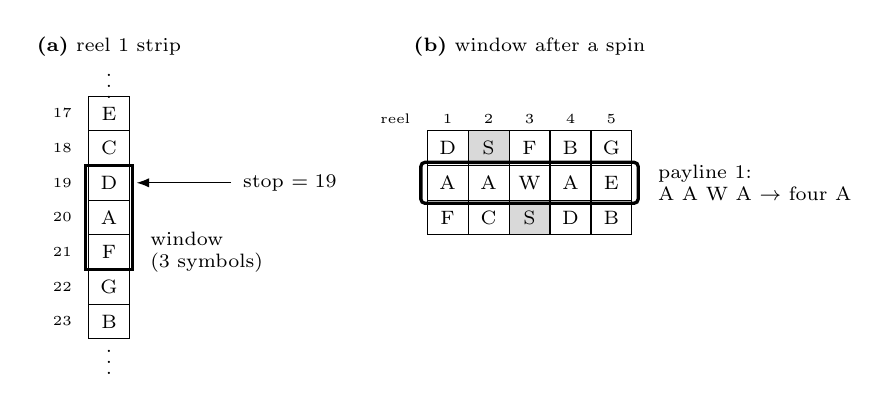
\begin{tikzpicture}[
    font=\scriptsize,
    cell/.style={draw, minimum width=5.2mm, minimum height=4.4mm, inner sep=0pt},
    scat/.style={cell, fill=black!15},
  ]
  % ---- (a) one reel strip ----
  \node at (0,2.55) {\textbf{(a)} reel 1 strip};
  \node at (0,2.15) {$\vdots$};
  \foreach \y/\pos/\sym in {1.70/17/E, 1.26/18/C, 0.82/19/D, 0.38/20/A, -0.06/21/F, -0.50/22/G, -0.94/23/B}{
    \node[cell] at (0,\y) {\sym};
    \node[anchor=east] at (-0.35,\y) {\tiny\pos};
  }
  \node at (0,-1.35) {$\vdots$};
  \draw[very thick] (-0.30,1.04) rectangle (0.30,-0.28);
  \node[anchor=west, align=left] at (0.40,-0.06) {window\\(3 symbols)};
  \draw[-{Latex[length=1.6mm]}] (1.55,0.82) -- (0.35,0.82);
  \node[anchor=west] at (1.58,0.82) {stop $= 19$};

  % ---- (b) the 3x5 window ----
  \begin{scope}[xshift=4.3cm, yshift=0.38cm]
    \node at (1.04,2.17) {\textbf{(b)} window after a spin};
    \node[anchor=east] at (-0.35,1.25) {\tiny reel};
    \foreach \c in {0,...,4}{
      \node at (0.52*\c,1.25) {\tiny \the\numexpr\c+1\relax};
    }
    % row 0
    \node[cell] at (0.00, 0.88) {D}; \node[scat] at (0.52, 0.88) {S};
    \node[cell] at (1.04, 0.88) {F}; \node[cell] at (1.56, 0.88) {B};
    \node[cell] at (2.08, 0.88) {G};
    % row 1
    \node[cell] at (0.00, 0.44) {A}; \node[cell] at (0.52, 0.44) {A};
    \node[cell] at (1.04, 0.44) {W}; \node[cell] at (1.56, 0.44) {A};
    \node[cell] at (2.08, 0.44) {E};
    % row 2
    \node[cell] at (0.00, 0.00) {F}; \node[cell] at (0.52, 0.00) {C};
    \node[scat] at (1.04, 0.00) {S}; \node[cell] at (1.56, 0.00) {D};
    \node[cell] at (2.08, 0.00) {B};
    % payline 1 (middle row)
    \draw[very thick, rounded corners=1.5pt] (-0.34,0.70) rectangle (2.42,0.18);
    \node[anchor=west, align=left] at (2.55,0.44) {payline 1:\\A A W A $\to$ four A};
  \end{scope}
\end{tikzpicture}
\caption{(a) A spin picks a stop on each strip; the window shows that symbol and the next two. (b) The resulting window. On payline~1 the wild~W completes a run of four A's, which pays 100 line bets. Only two scatters (shaded) are visible, so no free games start.}
\label{fig:reels}
\end{figure}

\paragraph{How a spin pays.}
The total bet $B$ is divided over 20 paylines, hence the line bet is $B/20$. Three or more of the same symbol in a row on a payline, counted from the leftmost reel, pays a prize multiplied by the line bet: 20, 100 or 200 for 3, 4 or 5 of A, B or C; 5, 20 or 100 for D or E; and 1, 10 or 50 for F or G. Besides these seven regular symbols there are two special symbols. The wild (W) can substitute for any regular symbol and has its own pays (40, 400 or 1000), and the higher prize is paid when both could pay on the same line. The scatter (S) pays anywhere in the window, at 10, 50 or 500 times the total bet for 3, 4 or 5 scatters. The win of a single spin is capped at $1100B$.

\paragraph{Free games.}
Three or more scatters anywhere in the window award 10 free spins, played at no extra cost on a separate free reel set, so mathematicians have to manage two reel sets: base and free. Scatters inside the free spins award 10 additional free spins, hence a \emph{retrigger}, so the number of free spins in a round is not fixed.

\paragraph{Stats a mathematician has to maintain.}
\emph{Return to player} (RTP) is the average amount paid back to the player: a game with an RTP of 95\% pays back 95 dollars for every 100 dollars staked, on average. Total RTP consists of base-game RTP and free-game RTP, both counted per base spin, and our game has a target of 0.95 (0.57 base and 0.38 free). \emph{Hit rate} is quoted as ``1 in $X$'', i.e.\ on average one in every $X$ spins wins something; for a fixed RTP, a larger $X$ means less frequent but bigger wins. \emph{Trigger rate} is the number of base spins per free-game trigger, and \emph{retrigger rate} the number of free spins per retrigger, both also quoted as ``1 in $X$''. These stats are recorded in the game's PAR sheet~\cite{harrigan2009par}. RTP is the number regulators check, and the same game can be released with different RTPs, each with a different reel set~\cite{harrigan2010tight}.

Reel sets are tuned manually by mathematicians: they change the frequency and position of symbols on each strip, run several million simulated spins, check the results and redo the whole process until the desired result is achieved. No change touches only one stat: an extra wild can raise both RTP and hit rate, and an extra scatter makes free games come more often, adds scatter prizes and so raises the overall RTP.


% ---------------------------------------------------------------------
\section{Related Work}
\label{sec:related}
\chk{Section 3: search-based game balancing and PCG; evolutionary optimisation under noise; slot reel-strip and RTP design; steady-state vs generational GAs and takeover time.}

% =====================================================================
%  Section 4 - Problem formulation (author's 4.1-4.2, edited; 4.3-4.4 in the same voice)
% =====================================================================
\section{Problem Formulation}
\label{sec:problem}

\subsection{Search Space and Two Tuning Stages}
\label{sec:space}

A candidate solution is one reel set $x = (r_1, \dots, r_5)$, where each strip $r_j \in \Sigma^{L}$ holds $L = 50$ symbols from the 9 symbols $\Sigma = \{\mathrm{A}, \dots, \mathrm{G}, \mathrm{W}, \mathrm{S}\}$. We put no constraint on symbol counts, so a strip can hold any number of copies of a symbol, or none.

The base and free reels are tuned separately, first the base reels and then the free reels. During the base stage, the three base stats (base RTP, hit rate and trigger rate) are calculated and tuned. For the free stage the base reels are fixed and only the free reel set changes. The three free stats are free RTP, free hit rate and retrigger rate. Free RTP also depends on the base trigger rate $T$, but keeping the base reels constant makes it depend only on the free reels.

\subsection{Objective}
\label{sec:objective}

Each stage has three stats $s_i(x)$, each with a target $t_i$ and a weight $w_i$ (Table~\ref{tab:targets}), and we minimise the weighted sum of relative errors
\begin{equation}
  F(x) \;=\; \sum_{i} w_i \, \frac{\lvert s_i(x) - t_i \rvert}{t_i}\,.
  \label{eq:fitness}
\end{equation}
$F(x) = 0$ means every target stat is matched exactly. Dividing the error of each stat by its target normalises it, so that stats on very different scales, such as an RTP of 0.57 and a trigger rate of 80, can be added together. Rates enter in their ``1 in $X$'' form. RTP has the highest weight, since it is the value that testing labs and licensing bodies check, whereas the trigger rate has more room: being 15 or more spins away from the target can be acceptable. A weighted sum is the simplest way to combine several targets and is close to how a mathematician reads a PAR sheet, but it hides the trade-off when targets conflict, which happens in the free stage (Sect.~\ref{sec:results}).

\begin{table}[t]
\centering
\caption{Targets $t_i$ and, in brackets, weights $w_i$ of the objective~\eqref{eq:fitness}. Rates are ``1 in $X$''; the free stage has a retrigger rate.}
\label{tab:targets}
\begin{tabular}{@{}lccc@{}}
\toprule
Stage & RTP & Hit rate & (Re)trigger rate \\
\midrule
Base & 0.57 (10) & 3 (6)   & 80 (3) \\
Free & 0.38 (10) & 2.7 (6) & 60 (3) \\
\bottomrule
\end{tabular}
\end{table}

\subsection{Noisy Evaluation by Simulation}
\label{sec:noise}

For this game, every stat could actually be calculated exactly: line-win RTP follows from the symbol counts on each reel, hit rate from going through all $50^5$ windows, and the free game from a geometric series over the number of free spins. However, we want a tuning process that also works for cascade and cluster games, where exact maths becomes much harder. Hence, the same way mathematicians check reel sets, we treat the game as a black box and use a multithreaded C++ Monte Carlo simulator. One evaluation plays $n = 10^7$ base spins with a random seed $\omega$ and returns $\hat F_n(x;\omega)$, which takes about 0.15\,s on 10 threads. In the free stage, the trigger rate $T$ of the fixed base reels is measured once from $10^8$ spins, and each evaluation then plays $\mathrm{round}(10^7/T)$ free rounds directly, i.e.\ the number of rounds a $10^7$-spin full game would play on average, and free RTP is calculated by dividing by $T$. This skips the base spins between free rounds and saves simulation time.

Since every stat comes from a finite number of spins, the score is noisy. Every evaluation in a run uses the same seed $\omega$ (common random numbers~\cite{law2015simulation}), so the same reel set always gets the same score, and a reel set that got a lucky score keeps it. The standard deviation of one $10^7$-spin estimate of $F$ is around 0.013 for good base reel sets and 0.035 in the free stage (Sect.~\ref{sec:noisestudy}), which near the end of the base stage is close to the gap between good candidates. A run also reports the lowest of about 1000 noisy scores, which favours the reel set whose noise was lucky~\cite{jin2005evolutionary,rakshit2017noisy}. So for every result we report, we re-evaluated the run's best reel set with $10^8$ spins on a seed the run never used (Sect.~\ref{sec:reeval}).

\subsection{Initialisation and Variation Operators}
\label{sec:operators}

A random reel set puts one copy of every symbol on each strip, fills the other 41 positions at random and shuffles the strip. Mutation picks $m \in \{1, 3, 5, 10\}$ of the 250 positions without replacement and changes each one to a different random symbol. The GA, hill climbing and simulated annealing all use this same mutation, so any difference between them comes from the population, crossover and the acceptance rule. Crossover works reel by reel: for each reel a cut point $c \in \{1, \dots, L-1\}$ is drawn, and the child takes the first $c$ symbols from one parent and the rest from the other. Every child gets crossover first and then mutation.


% =====================================================================
%  Section 5 - Methods (author's 5.1-5.2, edited)
% =====================================================================
\section{Methods}
\label{sec:methods}

We compare twelve methods: nine GA configurations (three replacement schemes $\times$ three selection operators) and three baselines, i.e.\ random search, hill climbing and simulated annealing (Table~\ref{tab:methods}). All twelve use the same representation, initialisation and mutation (Sect.~\ref{sec:operators}), the same objective (Sect.~\ref{sec:objective}) and the same budget of 1000 evaluations.

\begin{table}[t]
\centering
\caption{The twelve methods. $\mu$ is the population size. ``Per step'' is one generation or iteration. Every method spends exactly 1000 evaluations.}
\label{tab:methods}
\setlength{\tabcolsep}{4pt}
\small
\begin{tabular}{@{}llcclc@{}}
\toprule
Method & Selection & $\mu$ & Per step & Survivors & Steps \\
\midrule
Steady-state GA     & T / R / SUS & 10 & 2 $\to$ 1   & replaces the worst if better & 1000 \\
Elitist gen.\ GA    & T / R / SUS & 10 & 8 $\to$ 8   & 2 best + 8 children                & 125 \\
Generational GA     & T / R / SUS & 10 & 10 $\to$ 10 & 10 children                        & 100 \\
\midrule
Hill climbing       & --- & 1 & 1 $\to$ 1 & child, if not worse                           & 1000 \\
Simulated annealing & --- & 1 & 1 $\to$ 1 & if better, else prob.\ $e^{-\Delta/\tau}$ & 1000 \\
Random search       & --- & 1 & 0 $\to$ 1 & best so far                                   & 1000 \\
\bottomrule
\multicolumn{6}{@{}p{\linewidth}@{}}{\footnotesize T = tournament ($k=3$), R = rank-based roulette wheel, SUS = stochastic universal sampling. ``$a \to b$'': $a$ parents selected, $b$ children evaluated.}
\end{tabular}
\end{table}

\subsection{The Genetic Algorithm}
\label{sec:ga}

The GA starts with 10 random reel sets, the same 10 for every GA combination and for the baselines, and each of them is evaluated once. In each generation, parents are selected, children are created by crossover, each child is mutated and evaluated, and then it is decided which members of the population are replaced. The GA keeps track of the best reel set it has seen so far, since a scheme such as generational replacement can lose its best member.

\paragraph{Selection.}
All three selection methods only consider the ranking of the population, not the size of the errors, because $F$ is around 90 or more at the beginning and falls below 0.1 at the end, so fitness-proportional selection would work very differently at the start and at the end of a run. \emph{Tournament} ($k = 3$) draws three distinct members at random and selects the best; each parent comes from its own tournament. \emph{Roulette} uses Baker's linear ranking~\cite{baker1985adaptive} with selection pressure $s = 2$, so the best member gets a weight of 2 and the worst a weight of 0, and chooses a single parent per spin. \emph{SUS}~\cite{baker1987reducing} uses the same weights, but places $n$ pointers $\mu/n$ apart from a single random start, where $n$ is the number of parents. So even though Roulette and SUS have the same expected selection count, Roulette can by chance leave the best member out entirely, whereas SUS always selects it when 8 or 10 parents are drawn.

\paragraph{Replacement.}
The three schemes range from replacing a single worst member to replacing all the members~\cite{dejong1993generation}. \emph{Steady-state} selects 2 parents and produces a single child, which replaces the worst member if it is strictly better, hence the best member is never lost~\cite{whitley1989genitor,syswerda1991study}. \emph{Generational} selects 10 parents and pairs them, each pair creates two children, and the 10 children replace the whole population, hence the best genes can be lost. \emph{Elitist generational} copies the 2 best members as they are and replaces the other 8 by 8 children of 8 parents selected from the whole population.

\subsection{Baselines}
\label{sec:baselines}

\paragraph{Random search} draws a new random reel set at every evaluation and keeps the best. It uses no mutation, so it is run once per seed and reported under every mutation strength.

\paragraph{Hill climbing} is the (1+1)~EA~\cite{droste2002analysis}. It takes the best reel set among the initial 10, mutates it, and replaces it with the child if the child is at least as good. Apart from accepting ties, hill climbing is the same as a steady-state GA with a population of 1 and no crossover. That makes it the main baseline the GA has to beat: since both use the same mutation, beating hill climbing shows that the population and crossover give an advantage in tuning.

\paragraph{Simulated annealing}~\cite{kirkpatrick1983optimization} is the same as hill climbing, but it can also accept a worse child $y$ of the current reel set $x$, with probability $\exp(-\Delta/\tau)$, where $\Delta = \ln \hat F(y) - \ln \hat F(x)$. The log scale is used because the score falls by about three orders of magnitude during a run, so on a linear scale a fixed temperature would either accept far too much at the end or almost nothing at the beginning. The temperature falls geometrically from $\tau_0 = 0.14$ at the first evaluation to $\tau_{\mathrm{end}} = 0.002$ at the last, and the method returns the best reel set it has seen.

\subsection{Equal Budgets and Parameter Choices}
\label{sec:fairness}

\paragraph{Same budget.} Every method spends exactly 1000 evaluations after the initial population (Table~\ref{tab:methods}). In the base stage and the fixed-base check, the ten evaluations of the initial population are made once per seed and shared; in the main free stage each method re-evaluates them on its own base reels. The GA starts from all ten and the baselines from the best of them. In the base stage every evaluation plays exactly $10^7$ spins. In the free stage each evaluation plays $\mathrm{round}(10^7/T)$ free rounds, which differs between methods, since each method's free stage uses the base reels that method found: a median of about 125{,}500 rounds for the GA and local-search methods, but about 560{,}000 for random search, whose base reels trigger free games about every 18 spins instead of every 80. The fixed-base check of Sect.~\ref{sec:reeval} removes this difference.

\paragraph{Parameters.} No method was tuned. The GA settings ($\mu = 10$, $k = 3$, $s = 2$, two elites, crossover on every child) are common textbook defaults~\cite{eiben2015introduction}. The annealing temperatures were set once, when the baselines were added to the code, and were not changed afterwards: at $\tau_0 = 0.14$ a child 10\% worse is accepted with probability $\exp(-\ln 1.1/0.14) \approx 0.51$, and at $\tau_{\mathrm{end}} = 0.002$ even a child 1\% worse is accepted with probability below 0.01, so the search ends as a hill climber. So the comparison is between sensible default settings, not between methods each tuned to its limit (Sect.~\ref{sec:discussion}).


% =====================================================================
%  Section 6 - Experimental setup (author's edits in 6.2-6.4)
% =====================================================================
\section{Experimental Setup}
\label{sec:setup}

\subsection{Design}
\label{sec:design}

Every method was run on 30 seeds at each of the four mutation strengths $m \in \{1, 3, 5, 10\}$. Random search does not use mutation, hence it is run once per seed and stage, which gives 1{,}350 runs per stage. Each seed runs the base stage first and then the free stage, where the free stage of each method uses the base reels that method found. During the base stage free games are triggered and counted for the trigger rate, but not played, since the free reels are still random at that point. For each seed, every method starts from the same 10 random reel sets and uses the same simulator seed for every evaluation, the same mutation operator and strength, and the same budget, so on any seed, all twelve methods face exactly the same problem, and all the tests below compare methods seed by seed. Every random number in a run is derived from the seed number, so any run can be repeated exactly.

\paragraph{Computing.} A run of 1000 evaluations plus its re-evaluation takes about 2.5 minutes on 10 threads, and the main study took 83 run-hours, about 14 hours on a 64-core machine running 6 seeds in parallel. The code, the results and the simulator are available at \url{https://osf.io/bw32t/overview?view_only=06e35aa867254e2da2c94bcfc0450f67}.

\subsection{Re-evaluation and Fixed-Base Check}
\label{sec:reeval}

As explained in Sect.~\ref{sec:noise}, the best score seen inside a run is optimistic. Hence the best reel set of every run is re-simulated with $10^8$ spins, i.e.\ ten times the spins of one evaluation, on a seed the run never used. In the base stage this re-evaluation plays the base game only, and in the free stage it plays the full game. Every error we report in Sect.~\ref{sec:results} is this re-evaluated value.

In the free stage, each method was run using the best base reel set found during its own base-stage run, which can make the free-stage comparison unfair, as some methods start with worse base reels than others. To make the comparison fair, all methods were later run again using the same fixed base reel set, the best one found over all base-stage runs. This fixed-base check covers $m \in \{3, 5, 10\}$ and all eleven methods other than random search, i.e.\ $30 \times 3 \times 11 = 990$ runs. Random search was left out because it is already far behind every other method in the free stage (median error 62.8, against about 1.6 at $m = 3$) and its fully random free reels make every evaluation slow.

\subsection{Statistical Tests}
\label{sec:stats}

Methods are compared in families, separately for each mutation strength: the three replacement schemes (per seed, the median over their three selection methods), the three selection methods inside each replacement scheme, the nine GA configurations against the three baselines, and the mutation strengths inside each method. Pairs are compared with two-sided Wilcoxon signed-rank tests paired by seed, with Holm correction inside the family and $\alpha = 0.05$. We also report a Friedman test per family, but since Holm correction already controls the chance of any false positive in the family, the pairwise results are not made conditional on it. As effect size we report the Vargha--Delaney $A_{12}$, i.e.\ the probability that one method ends with a lower error than the other on a run, where 0.5 means no difference, with the usual bands: negligible below 0.56, small from 0.56, medium from 0.64 and large from 0.71.

Some differences can be significant and still smaller than what the simulator can measure. Two independent measurements have to differ by $1.96\sqrt{2} \approx 2.77$ standard deviations to be told apart at 95\%. For the noise floor we use a standard deviation of 0.034 for the base stage and 0.10 for the free stage at $10^7$ spins, fixed from an earlier noise measurement before the main experiment. Both are above the largest values in the final noise study (0.030 and 0.093 for random search's reel sets, 0.025 and 0.061 for the other methods), so the floor is conservative. This gives floors of $2.77 \times 0.034/\sqrt{10} = 0.0298$ and $2.77 \times 0.10/\sqrt{10} = 0.088$ at the $10^8$ spins of the re-evaluation. A difference counts as a finding only if it is significant after Holm correction, its $A_{12}$ is at least small, and the gap between the medians is above the noise floor.


% =====================================================================
%  Section 7 - Results (author's edits in 7.1-7.5)
%  Every number below is from Results/stats/*, NoiseStudy/report.txt
%  and the released results.json / results_fixedbase.json.
% =====================================================================
\section{Results}
\label{sec:results}

All errors in this section are re-evaluated errors (Sect.~\ref{sec:reeval}), given as medians over the 30 seeds, and lower is better. Table~\ref{tab:main} gives every method at every mutation strength for both stages.

\begin{table}[!htb]
\centering
\caption{Median re-evaluated error over 30 seeds (lower is better). SS = steady-state, EL = elitist generational, GEN = generational. Bold: within one noise floor of the best value in its column (0.0298 base, 0.088 free, Sect.~\ref{sec:stats}).}
\label{tab:main}
\setlength{\tabcolsep}{3.5pt}
\footnotesize
\begin{tabular}{@{}lcccccccc@{}}
\toprule
 & \multicolumn{4}{c}{Base stage, $m =$} & \multicolumn{4}{c}{Free stage, $m =$} \\
\cmidrule(lr){2-5}\cmidrule(l){6-9}
Method & 1 & 3 & 5 & 10 & 1 & 3 & 5 & 10 \\
\midrule
SS + Tournament & \textbf{0.076} & \textbf{0.114} & \textbf{0.090} & \textbf{0.139} & 2.032 & \textbf{1.303} & 1.347 & 1.797 \\
SS + Roulette & 0.163 & 0.137 & 0.150 & 0.206 & 2.008 & 1.356 & 1.718 & 1.766 \\
SS + SUS & 0.140 & 0.153 & \textbf{0.091} & 0.169 & 2.072 & \textbf{1.262} & 1.489 & 1.593 \\
EL + Tournament & 0.176 & 0.119 & \textbf{0.100} & 0.210 & 2.021 & 1.423 & \textbf{1.174} & 1.601 \\
EL + Roulette & 0.155 & \textbf{0.086} & 0.132 & 0.269 & 1.940 & 1.363 & 1.474 & \textbf{1.574} \\
EL + SUS & 0.135 & 0.151 & 0.148 & 0.221 & \textbf{1.828} & 1.479 & 1.431 & 1.730 \\
GEN + Tournament & 0.169 & 0.158 & 0.209 & 0.522 & 2.010 & 1.706 & 1.870 & 1.990 \\
GEN + Roulette & 0.252 & 0.349 & 0.445 & 1.555 & 2.069 & 1.907 & 2.001 & 2.059 \\
GEN + SUS & 0.173 & 0.234 & 0.333 & 0.830 & \textbf{1.885} & 1.729 & 1.900 & 1.952 \\
\midrule
Hill climbing & 0.160 & 0.118 & \textbf{0.084} & \textbf{0.128} & 1.988 & 1.780 & 1.559 & \textbf{1.527} \\
Simulated annealing & 0.192 & 0.130 & \textbf{0.075} & \textbf{0.155} & 1.926 & 1.532 & 1.277 & \textbf{1.494} \\
Random search & 37.5 & 37.5 & 37.5 & 37.5 & 62.8 & 62.8 & 62.8 & 62.8 \\
\bottomrule
\end{tabular}
\end{table}

\subsection{Automatic Tuning Works}
\label{sec:res-works}

In the base stage, the best of the 10 random starting reel sets has a median error of about 97. With 1000 evaluations, every method except random search brings this down to between 0.075 and 0.25 at its best mutation strength, and most of them to around 0.1 (Table~\ref{tab:main}). An error of 0.1 means, for example, a base RTP that is 1\% off its target with the other two stats exact. Random search, with the same budget, stays at 37.5 and loses to every GA configuration on 30 of 30 seeds at every mutation strength ($p_{\mathrm{Holm}} < 0.001$, $A_{12} = 1.00$), so the result comes from the search itself and not from luck.

\subsection{Replacement, Selection and Mutation}
\label{sec:res-ga}

\paragraph{Replacement decides the result.} Generational replacement is the worst scheme, and the gap grows with mutation strength. Against steady-state, its median error is 0.185 vs 0.145 at $m = 1$, 0.214 vs 0.144 at $m = 3$, 0.333 vs 0.144 at $m = 5$ and 0.707 vs 0.162 at $m = 10$, where it loses on 30 of 30 seeds ($A_{12} = 1.00$, $p_{\mathrm{Holm}} < 0.001$). Elitist replacement beats generational in the same way from $m = 3$ upwards. The result at $m = 1$ is the weakest one ($p_{\mathrm{Holm}} = 0.044$, Friedman $p = 0.107$). Steady-state and elitist replacement are tied at $m = 1$, 3 and 5. Only at $m = 10$ is steady-state better (0.162 vs 0.224, $p_{\mathrm{Holm}} = 0.007$, $A_{12} = 0.72$).

\paragraph{Selection matters only without elitism.} Inside steady-state and inside elitist replacement, no pair of selection methods differs significantly at any mutation strength. Inside generational replacement, selection does matter: Tournament beats Roulette at every $m$, SUS beats Roulette at every $m$, and Tournament beats SUS from $m = 3$ upwards.

\paragraph{Gentle mutation is better.} Changing 10 of the 250 positions is significantly worse than a smaller $m$ for 9 of the 11 methods. The damage is largest for generational replacement: Generational + Roulette goes from 0.252 at $m = 1$ to 1.555 at $m = 10$.
\subsection{GA versus Local Search}
\label{sec:res-baselines}

In the base stage, no GA configuration is significantly better than hill climbing or simulated annealing at any mutation strength. With each method at its own best mutation strength, the best GA (SS + Tournament, $m = 1$) and simulated annealing ($m = 5$) reach 0.076 and 0.075, simulated annealing is lower on 15 of the 30 seeds, $A_{12} = 0.53$ and $p_{\mathrm{Holm}} = 1.0$, i.e.\ a draw.
In the other direction, the baselines are significantly better than every generational configuration at $m = 5$ and 10, so in the base stage the best a well-configured GA can do is a draw, and a badly configured GA loses to local search.

\subsection{Free Game and Fixed-Base Check}
\label{sec:res-free}

The free stage has a higher error, with best medians of 1.17 to 1.30 against about 0.1 in the base stage, because the free-game targets pull against each other (Fig.~\ref{fig:tradeoff}). The ranking of methods is similar: steady-state and elitist replacement are at the top, level with simulated annealing, and generational replacement is significantly worse than both at $m = 3$, 5 and 10 ($A_{12}$ from 0.80 to 0.94). Three things differ. First, $m = 1$ is now the worst mutation strength for 10 of the 11 methods. Second, elitist replacement beats steady-state at $m = 1$ and 5 ($p_{\mathrm{Holm}} = 0.030$ and 0.009, $A_{12} = 0.65$). Third, all six steady-state and elitist configurations beat hill climbing at $m = 3$, e.g.\ SS + SUS with 1.262 vs 1.780 on 27 of 30 seeds ($A_{12} = 0.83$, $p_{\mathrm{Holm}} < 0.001$), whereas no GA configuration beats simulated annealing at any $m$. Selection again matters mainly inside generational replacement (one exception: EL + SUS beat EL + Tournament at $m = 1$, $p_{\mathrm{Holm}} = 0.034$).

With the fixed base reels, the median error over the 990 paired runs barely moves (1.661 vs 1.649, Wilcoxon $p = 0.77$), the ranking is kept (Spearman $\rho = 0.84$), and the same findings hold, except that only three configurations beat hill climbing at $m = 3$ (SS + SUS, SS + Tournament and EL + SUS). So the free-stage findings do not come from the base reels.

\begin{figure}[t]
\centering
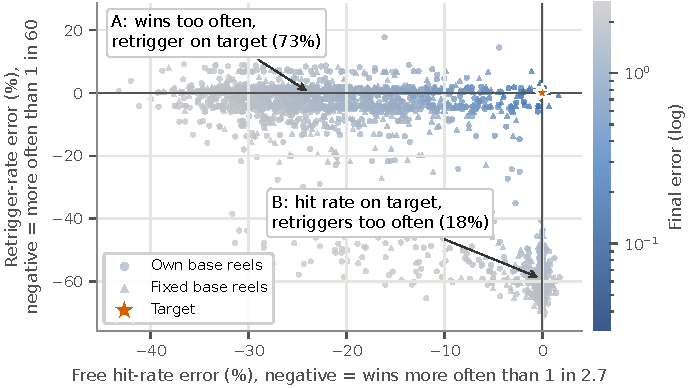
\includegraphics[width=\textwidth]{figures/free_tradeoff.pdf}
\caption{Free stage: error in free hit rate against error in retrigger rate (in \%) for the 2310 final free reel sets, with each method's own base reels (circles) and with the fixed base reels (triangles), random search excluded. Colour shows the final error; the target is the star at (0, 0). Most reel sets fall into two groups: A hits the retrigger target but wins too often, and B hits the hit-rate target but retriggers too often.}
\label{fig:tradeoff}
\end{figure}

Of the 2310 final free reel sets, 73\% hit the retrigger target but win too often, 18\% hit the free hit-rate target but retrigger far too often, and only 16 (0.7\%) reach an error of 0.25 or less. Every retrigger adds 10 spins, so more retriggers mean longer rounds and more free RTP. With this game's symbols and rules the free-game targets appear to conflict, and every method has to trade one against the other.

\subsection{Noise Study}
\label{sec:noisestudy}

Re-simulating the best reel sets 30 times each with $10^7$ spins, the standard deviation of the error is about 0.013 in the base stage and 0.035 in the free stage (medians over reel sets), almost the same for every method except random search, since it comes from the simulator and not from the optimiser. For a given method and $m$, the spread of final errors between seeds (interquartile range) is a median 4.3 times the noise floor in the base stage and 5.6 times in the free stage, so the outcome of a run is decided by the search, not by measurement error. The in-run best is optimistic: in the base stage the re-evaluated median is higher than the in-run median in 36 of 44 method--mutation combinations (median ratio 1.04), and in one case by a factor of 1.63 (SS + Tournament at $m = 1$: 0.047 during the run, 0.076 on re-evaluation); in the free stage the ratios lie between 0.98 and 1.07.
Finally, every significant difference reported above is also larger than the noise floor: all 75 in the base stage, 67 in the free stage and 27 in the fixed-base check. However, noise does limit the order among the best GA configurations and the baselines, as their differences are within the noise floor in the base stage, and that is why they are reported as tied rather than ranked.


% =====================================================================
%  Section 8 - Discussion and threats to validity (author's version,
%  facts checked against Sects. 4-7 and NoiseStudy/report.txt)
% =====================================================================
\section{Discussion and Threats to Validity}
\label{sec:discussion}

\paragraph{Why generational replacement fails.} Generational replacement replaces all the parents, meaning no reel set survives unchanged. Near the end of a run, when the reel sets are close to the targets, the children are mostly worse than their parents, and a higher mutation strength has a more severe impact. Unlike generational replacement, steady-state and elitist replacement never lose the best reel set, so a bad child costs just one evaluation, nothing more.

\paragraph{Selection only matters when replacement does not keep the best.} With steady-state and elitist replacement the best reel sets are always kept, but with generational replacement, selection is the only way good reel strips reach the next generation. When 10 parents are drawn from 10 members, Tournament ($k = 3$) picks the best member 3 times on average and misses it in $0.7^{10} \approx 3\%$ of generations. SUS picks it exactly twice. Roulette also picks it twice on average, but misses it in $0.8^{10} \approx 11\%$ of generations.
\paragraph{In the base stage, local search is enough.} Hill climbing is a steady-state GA with one member and no crossover (Sect.~\ref{sec:baselines}), so the only way the GA can beat it is if crossover or the population helps, but in the base stage neither did. Line-win RTP depends only on how many of each symbol a reel strip holds (Sect.~\ref{sec:noise}), and one mutation changes two of these counts by 1 in 50. So even without crossover, a chain of small mutation steps lowers the error. We think crossover adds very little near the end, but we never measured diversity or ran a GA without crossover.

\paragraph{In the free stage, a population and annealing help.} The free-game target stats conflict with each other (Sect.~\ref{sec:res-free}), so near the end every small change likely makes at least one of the stats worse. Since hill climbing only accepts a child that is not worse, it stays there. At $m = 3$ all six steady-state and elitist configurations beat it. Simulated annealing also works on a single reel set, but it accepts some worse children, and no GA configuration beats it at any $m$. So the gain seems to come from keeping or accepting reel sets other than the current best, which a population and annealing both do, and not from crossover.

\paragraph{Advice for slot mathematicians.} Start with a steady-state GA, an elitist GA or simulated annealing; all three reach a base error of about 0.1, e.g.\ a base RTP 1\% off its target. Do not use generational replacement without elitism. Changing 3 to 5 of the 250 symbols is a safe mutation strength for both stages. Also, re-simulate the final reel set with more spins on a new seed. Finally, if every good method stops at about the same error, as in our free stage (best medians 1.17 to 1.30), check the targets before changing the optimiser.

\paragraph{Threats to validity.} \emph{One game, one budget, one population size.} We tuned a simple line-win game against three stats per stage. More complex games may favour other methods. Every run had 1000 evaluations and $\mu = 10$. A larger budget might let crossover pay off, and a larger population gives more diversity but fewer generations; we tested neither. \emph{Untuned methods.} The GA used textbook defaults, and the annealing temperatures (0.14 to 0.002) were set once and never changed. Tuning could change the order among the tied methods, so our claim is about sensible defaults. \emph{Best $m$ chosen on the same seeds.} When each method is compared at its own best $m$, the same 30 seeds choose $m$ and measure the result. This favours the GA, whose best value is the lowest of 36 configurations (9 $\times$ 4 values of $m$) against 4 for simulated annealing. The base-stage draw holds despite this, and at a fixed $m = 5$ it is also a draw. \emph{Weighted-sum error and conflicting free targets.} The weights 10, 6 and 3 are our choice, and other weights could rank reel sets and methods differently. Only 16 of 2310 final free reel sets reach an error of 0.25 or less, so the free stage compares how methods trade one target against another. We did not prove that the free targets cannot all be met; the exact calculation of Sect.~\ref{sec:noise} could settle this. \emph{Noise floor.} Its standard deviations (0.034 and 0.10) come from a measurement made before the main experiment, and are above every value in the final noise study.

% ---------------------------------------------------------------------
\section{Conclusion}
\label{sec:conclusion}
\chk{Section 9, including multi-objective tuning of the free game as future work.}

% ---------------------------------------------------------------------
\subsubsection*{Use of AI Tools.}
\chk{Required statement: AI tools helped with the code, the analysis scripts and the writing.}

\bibliographystyle{splncs04}
\bibliography{refs}

\end{document}
